%%%%%%%%%%%%%%%%%%%%%%%%%%%%%%%%%%%%%%%%%%%%%
% PROCESAMIENTO DIGITAL DE SEÑALES DE AUDIO
% MAESTRÍA EN INGENIERÍA ELÉCTRICA, UDELAR
% SEGUNDO SEMESTRE 2016
%%%%%%%%%%%%%%%%%%%%%%%%%%%%%%%%%%%%%%%%%%%%%

%----------------------------------------------------------------------------------------
%	PACKAGES AND DOCUMENT CONFIGURATIONS
%----------------------------------------------------------------------------------------

\documentclass{article}

\usepackage[version=3]{mhchem} % Package for chemical equation typesetting
\usepackage{siunitx} % Provides the \SI{}{} and \si{} command for typesetting SI units

\usepackage[spanish]{babel}
\selectlanguage{spanish}
\usepackage[utf8]{inputenc}
\usepackage{graphicx} % Required for the inclusion of images
\usepackage{natbib} % Required to change bibliography style to APA
\usepackage{amsmath} % Required for some math elements 

\usepackage{float}

\usepackage{geometry}
 \geometry{
 a4paper,
 total={170mm,257mm},
 left=20mm,
 top=20mm,
 }

\usepackage{listings}
\usepackage{color} %red, green, blue, yellow, cyan, magenta, black, white
\definecolor{mygreen}{RGB}{28,172,0} % color values Red, Green, Blue
\definecolor{mylilas}{RGB}{170,55,241}

\lstset{language=Matlab,%
    %basicstyle=\color{red},
    breaklines=true,%
    morekeywords={matlab2tikz},
    keywordstyle=\color{blue},%
    morekeywords=[2]{1}, keywordstyle=[2]{\color{black}},
    identifierstyle=\color{black},%
    stringstyle=\color{mylilas},
    commentstyle=\color{mygreen},%
    showstringspaces=false,%without this there will be a symbol in the places where there is a space
    numbers=left,%
    numberstyle={\tiny \color{black}},% size of the numbers
    numbersep=9pt, % this defines how far the numbers are from the text
    emph=[1]{for,end,break},emphstyle=[1]\color{red}, %some words to emphasise
    %emph=[2]{word1,word2}, emphstyle=[2]{style},    
}

\setlength\parindent{0pt} % Removes all indentation from paragraphs

\renewcommand{\labelenumi}{\alph{enumi}.} % Make numbering in the enumerate environment by letter rather than number (e.g. section 6)


%----------------------------------------------------------------------------------------
%	DOCUMENT INFORMATION
%----------------------------------------------------------------------------------------

\title{\textbf{Extracción de embocadura en Aliento/Arrugas}\\\large \textsc{Proyecto Final - Procesamiento Digital de Señales de Audio - Curso 2016}\\
 \textsc{Maestría en Ingeniería Eléctrica} del \textit{Instituto de Ingeniería Eléctrica, Facultad de Ingeniería, Universidad de la República.}}

\author{\textit{Juan Braga}}
\date{\today}

\begin{document}

\maketitle 


\begin{abstract}
El presente trabajo tiene como objetivo principal la evaluación de características de diversa naturaleza, en la extracción automática de embocadura a partir de muestras de audio. Se trabaja sobre Aliento/Arrugas, obra para flauta con técnicas extendidas, del compositor contemporáneo Marcelo Toledo. 
\end{abstract}



%----------------------------------------------------------------------------------------
%	INTRODUCCIÓN
%----------------------------------------------------------------------------------------



\section{Introducción}

La Flauta traversa, perteneciente a la famila de \textit{Instrumentos de Madera}, es la única que no utiliza \textit{lengüeta} o \textit{caña} en su embocadura. Su mecanísmo de producción de la exitación periódica difiere del resto, ya que esta basado en la turbulencia generada por la colisión del flujo del aire con el bisel de su agüjero. La exitación periodíca pone a resonar a la columna de aire, y la altura es definida mediante la posición de las llaves del instrumento, característica que comparte con el resto de la familia de \textit{Maderas}. 
\medskip 

Además de la ejecución de alturas como material sonoro, los compositores académicos contemporáneos, exploran las capacidades sónicas del instrumento. Actualmente existen un montón de técnicas modernas, claramente definidas y reproducibles a las que se denominan extendidas. Diversos recursos técnicos forman parte del repertorio actual de la flauta y los intérpretes deben expandir sus habilidades con el instrumento.
\medskip

La extracción de contenido musical en este tipo de obras no se abarca solamente con estimación de alturas y duraciones, a diferencia del lenguaje tradicional de la flauta. El repertorio contemporáneo define un área del \textit{MIR} (por su sigla en inglés \textit{Music Information Retrieval}) desafiante y de espectro más amplio. Además es un área de estudio donde no existe mucho camino andando, habiendo tierra fértil para explorar y lograr contribuciones. 
\medskip

El cometido del presente trabajo es el acercamiento a este tipo de problemas, con objetivo la extracción automática de embocadura a partir de grabaciones de la obra contemporánea Aliento/Arrugas. En lo que sigue, Sección \ref{embocadura}, se define con más detalle el término embocadura, y se hace un análisis de sus principales implicancias en el sonido de la flauta. Además en la Sección \ref{aliento} se describe en mayor profunidad la pieza musical Aliento/Arrugas. Luego en la Seccion \ref{problema} se define el problema y la estrategia de resolucion, se detalla la base de datos y se da un breve marco teórico de las características a utilizar. La Sección \ref{experimento} esta dedicada a comentar los resultados y algunas consideraciones, para finalmente concluir el trabajo en el Sección \ref{conclusiones}. Por otro lado en el Anexo se puede ver una representación gráfica de las predicciónes para comparación visual con el ground truth.

\subsection{Embocadura}
\label{embocadura}
El término embocadura refiere al aparato de producción de la exitación de la columna de aire, en conjunto a la técnica de soplido \citep[Capítulo~6]{piston1955orchestration}. Por ejemplo en el caso particular de la flauta ejecutada con técnica tradicional, los labios dirigen el flujo de aire directamente al bisel en el hueco del instrumento. De esta forma la turbulencia producida por la colisión, genera una exitación periódica en la columna de aire que provoca la resonancia del instrumento y un sonido tonal. 
\medskip

La embocadura es un elemento determinante del material sonoro ejecutado, siendo perceptible de forma auditiva a través de variaciones en la dinámica, altura y timbre \citep[Capítulo~2]{dick1975other}. Las características sonoras quedan determinadas por los siguientes parámetros físicos de la ejecución del instrumento:

\begin{itemize}
  \item \textbf{Ángulo de la flauta:} Por un lado afecta la altura de la ejecución. Al girar hacia el intérprete la altura baja, por el contrario sube al girar en el otro sentido. Por otro lado genera cambios en el timbre del material sonoro. Al girar hacia afuera (sentido opuesto al intérprete) mas allá del ángulo normal de ejecución, el sonido se vuelve primero más brillante y luego aumenta la prominencia del componente de ruido, en inglés se lo define como \textit {Breathy}, se lo puede traducir al español como \textit{Respirado}. Sin embargo al girar hacia el intérprete aumenta la energía de los parciales altos y disminuye la fundamental generando un sonido que se puede definir metafóricamente como \textit{Filoso} o \textit{Edgy} por su denominación en inglés.
  \item \textbf{Apertura de los labios:} La apertura de los labios determina la dispersión del flujo de aire. Aperturas pequeñas producen flujos puntulaes, disminuyendo la dinámica y clarificando el sonido. Del otro lado aperturas mayores aumentan la intensidad y la naturaleza ruidosa.   
  \item \textbf{Posición de los labios:} Una posición correcta de los labios genera que la embocadura tenga gran control del sonido. Si bien la posición de los labios, y los movimientos de los mismos en la ejecución es un aspecto personal del ejecutante, existen dos tipos básicos. Alturas bajas y/o dinámicas intensas aumentan con el movimiento de los bordes de los labios hacia afuera generando casi una sonrisa en el intéprete. En la segunda posición de los labios, los bordes se mueven hacia abajo en vez de hacia afuera, teniendo un efecto similar al mencionado anteriormente.	
  \item \textbf{Presión de aire:} La presión de aire es controlada por el diafragma. Determina el nivel dinámico de la ejecución. La intensidad del aire es proporcional a la intensidad de la ejecución. Además afecta la altura del material sonoro, presiones de aire altas tienden a elevar la nota, mientras que presiones menores la disminuyen.	
\end{itemize}
\medskip 

\subsection{Aliento/Arrugas de Marcelo Toledo}
\label{aliento}
Aliento/Arrugas es una obra para flauta traversa solista, compuesta por el argentino Marcelo Toledo. Incluye una cantidad de sonoridades exóticas mediante la ejecución del insturmento a través de técnicas extendidas. Según el compositor la intención detrás es la exploración sonora del instrumento utilizando la respiración del intérprete como elemento de expresión orgánica \citep{candelaria2005argentine}.  
\medskip

El compositor utiliza como recurso expresivo tres tipos de embocadura para ejecución del instrumento. Se diferencian por cambios en la posición de los labios y el ángulo de la flauta (ver \ref{embocadura}), en otras palabras el ángulo entre el flujo de aire frente al bisel de la embocadura. Se enlista a continuación los nombres, manteniendo su denominación en Inglés (idioma utilizado en la partitura de la obra). Además en la Figura \ref{fig:embocaduras} se observa la notación utilizada por el compositor en la partitura de Aliento/Arrugas.

\begin{itemize}
  \item \textit{Normal Embouchure}: Embocadura clásica de la flauta, donde el flujo de aire frente al bisel de la embocadura genera la exitación con pulsos períodicos de la columna de aire. 
  \item \textit{Blow Hole Covert}: El flujo de aire ingresa directo al tubo de la flauta, sin generar turbulencia contra el bisel de la embocadura. Los labios cubren el agüjero del instrumento.
  \item \textit{Breathy Embouchure}: La flauta se encuentra rotada hacia el lado contrario del intérprete, tomando como referencia la embocadura normal. Genera sonidos con orientación tonal pero con un gran componente ruidoso.
\end{itemize}
\medskip

\begin{figure}[H]
\begin{center}
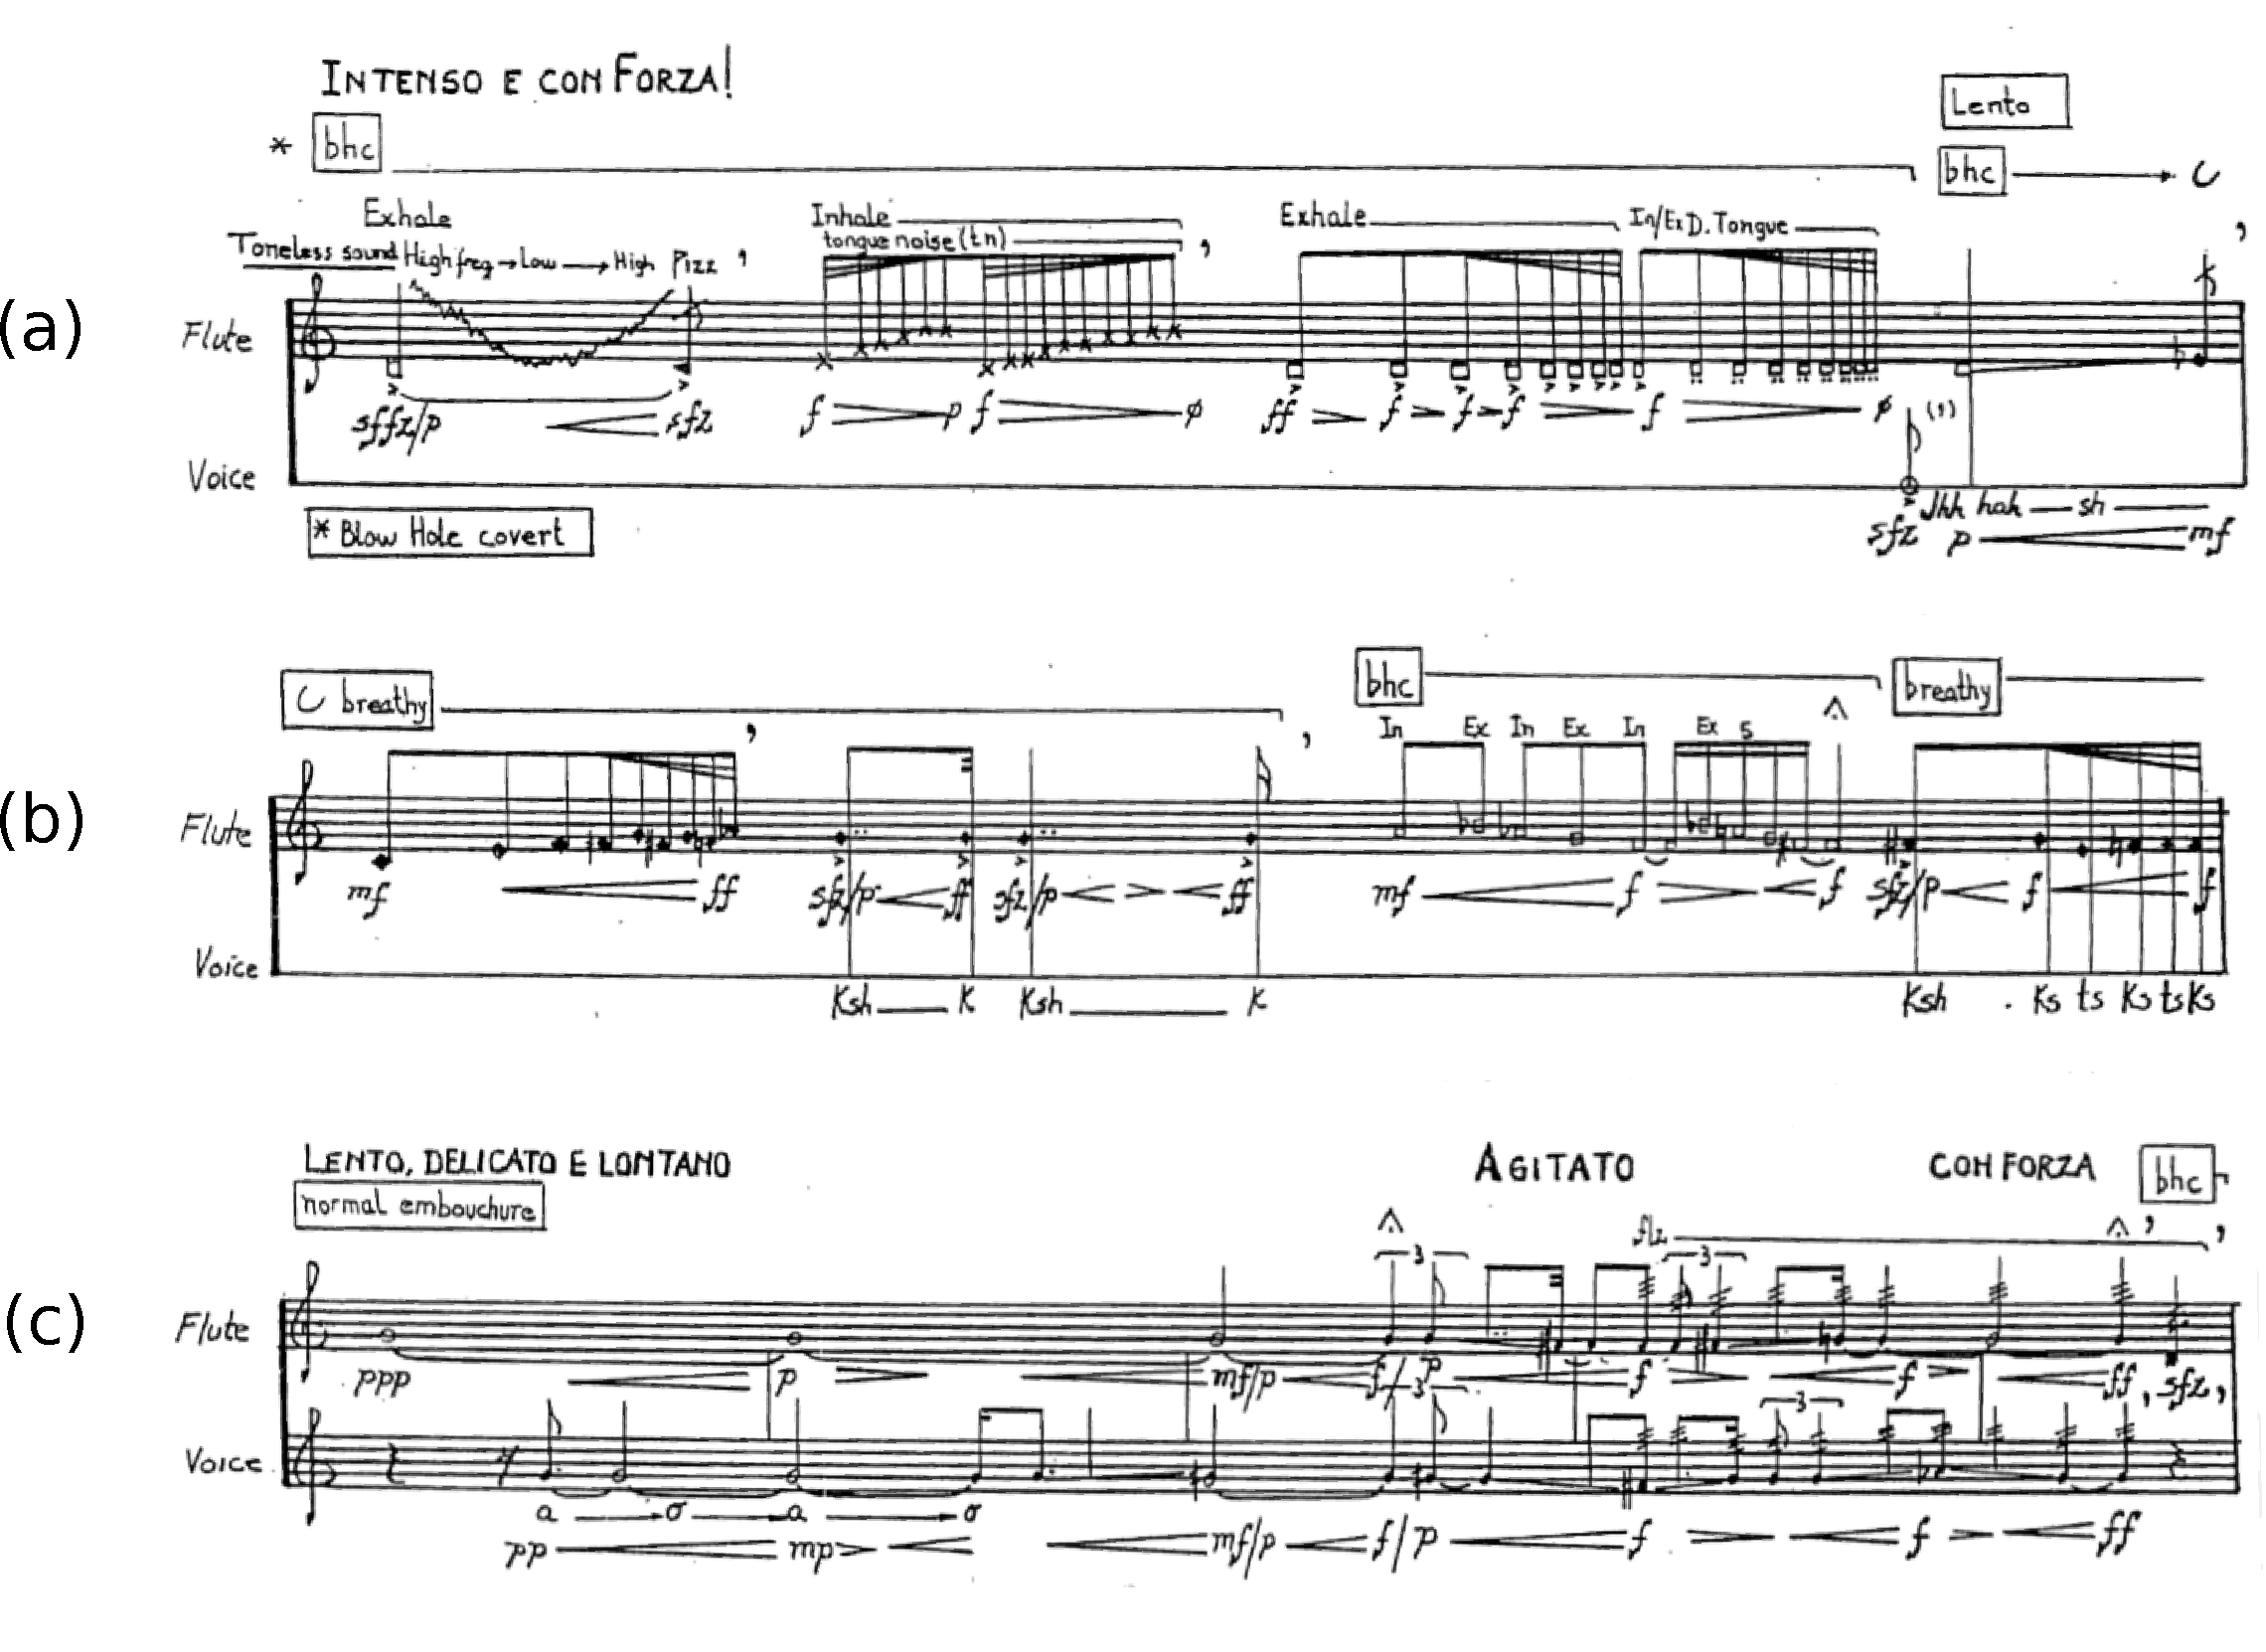
\includegraphics[width=0.5\textwidth]{embocaduras} 
\caption{Notación de las embocaduras se observa en la parte superior de los sistemas. (a) \textit{Blow Hole Covert}. (b) \textit{Breathy Embouchure}. (c) \textit{Normal Embouchure}. Fragmentos extraídos de la partitura de Aliento/Arrugas.}
\label{fig:embocaduras}
\end{center}
\end{figure}

\newpage

\section{Definición del Problema}
\label{problema}
Teniendo en cuenta que la embocadura es un elemento determinante del material sonoro ejecutado perceptible de forma auditiva (Sección \ref{embocadura}), se propone la extracción automática del tipo de embocadura a través del análisis computacional de grabaciones de la obra. 


\subsection{Estrategia de resolución}

Se propone la resolución del problema con un enfoque de reconocimiento de patrones. Se procesa el audio como un \textit{Bag of Frames} a partir del computo de descriptores numéricos. El principal desafío y cometido del presente trabajo es encontrar los descriptores que extraigan las diferencias en la naturaleza sonora y permitan la separación de las embocaduras en el espacio de características. 
\medskip

\subsection{Conjunto de Datos}
\label{datos}
Se cuenta con 5 grabaciones de diferentes intérpretes de la obra Aliento/Arrugas. Los intérpretes son: Pablo Somma, Emma Resmini, Claire Chase, Juan Pablo Quinteros y Ulla Suokko. Los archivos de audio se etiquetaron utilizando el software \textit{Sonic Visualiser} \citep{cannam2010sonic} dividiendo los archivos de audio en 5 clases:

\begin{itemize} 
  \item Silencio.
  \item Silencio con respiración del intérprete. 
  \item Sonido generado con \textit{Blow Hole Covert}.
  \item Sonido generado con \textit{Breathy Embouchure}.
  \item Sonido generado con \textit{Normal Embouchure}.
\end{itemize}

Las grabaciones de Claire Chase y Juan Pablo Quinteros que se obtuvieron para el presente trabajo sufrieron un proceso de compresión con pérdida, por lo que estos datos reciben un tratamiento distinto. No se utilizan para entrenar los algoritmos de clasificación, solo se utilizan como datos de test. Por lo que folds son de la siguiente forma: 



\begin{itemize} 
  \item Cuando la grabación de test es la de Ulla Suokko, Pablo Somma o Emma Resmini, se entrena con las otras dos restantes. Metodología de \textit{Leave One Out} por su demoninación en Inglés.
  \item Por otro lado cuando la grabación de test es de Claire Chase o Juan Pablo Quinteros, el conjunto de entrenamiento esta compuesto por las tres grabaciones sin pérdida (i.e. la de Ulla Suokko, Pablo Somma y Emma Resmini).
\end{itemize}

\begin{figure}[H]
\begin{center}
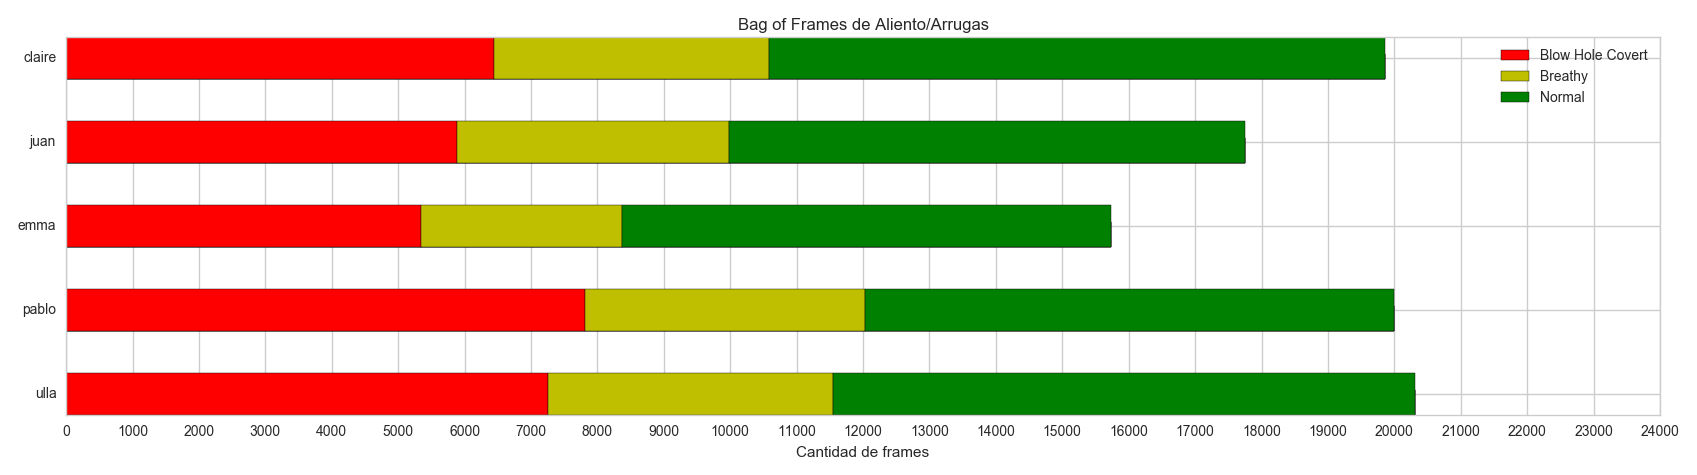
\includegraphics[width=1\textwidth]{dataset} 
\caption{Detalle de la composición del \textit{bag of frames} de embocaduras.}
\label{fig:dataset}
\end{center}
\end{figure}

En la Figura \ref{fig:dataset} se observa en detalle las cantidades de frames de embocaduras en la base de datos. Se puede observar según el intérprete la proporción de las clases. Se observa que la clase mayoritaria es la \textit{Normal embouchure} de numero comparable \textit{Blow Hole Covert} y sensiblemente menor es la dada por la embocadura \textit{Breathy}.

\medskip
En lo que sigue se utilizan únicamente las clases asociadas a cada una de las embocaduras. Queda por fuera del alcance de este trabajo, una etapa de pre-procesamiento para la segmentación del audio en fragmentos de actividad de la flauta y silencios (este problema se conocido como \textit{Activity Detection} por su denominación en Inglés). 
\medskip 


\subsection{Extracción de características}
\label{descriptores}
Se enlistan a continuación las características que se evalúan en la extracción automática de embocadura. Además se describe brevemente sus principales atributos.



\subsubsection{Mel-Frequency Cepstral Coefficients (MFCC)} 

Los \textit{Coeficientes Cepstrales de Frecuencia-Mel} fueron introducidos por \cite{davis1980comparison} en la resolución del problema de reconocimiento del hablante a partir de señales de voz (\textit{Speaker Recognition} su denominación en Inglés). Estos coeficientes como características de un sistema de reconocimiento automático del hablante han demostrado tener de los mejores desempeños \citep[Capítulo~14]{quatieri2002discrete}. A partir de ahí han sido utilizados en diversas problemáticas de clasificación que no involucran señales de voz hablada, con buenos resultados también como es el caso de reconocimiento de instrumentos \citep[Capítulo~6]{klapuri2007signal}. Su fortaleza radica en la incorporación del modelado psicoacústico de la audición humana mediante un banco de filtros basados en la escala Mel \citep{stevens1937scale} y la decorrleación que presentan los datos en el dominio de las \textit{quefrencys}, dado por la aplicación de la Transformada Coseno. Son un buen descriptor para la extracción de aspectos tímbricos de la señal.
\medskip

El cómputo de estas características cuenta con las etapas que se enlistan a continuación de manera conceptual: 

\begin{enumerate}
	\item División de la señal en fragmentos mediante enventanado.
	\item Cálculo de la magnitud de la Transformada discreta de Fourier de tiempo corto (STFT).
	\item Fitrado de la señal con banco de filtros Mel.
	\item Cálculo de la energía para cada filtro del banco.
	\item Logaritmo de las energías.
	\item Transformada Coseno de los valores a la salida del Logaritmo.
	\item \textit{Liftrado} de la señal resultante en el dominio de las \textit{quefrencys}, luego de la Transformada Coseno. Determina la cantidad de coeficientes, o en otras palabaras la dimensión del espacio de caracterísitcas.
\end{enumerate}

El cálculo de los coeficientes MFCC tiene los siguientes parámetros determinantes de su desempeño: En primer lugar el largo de las ventanas, que define el compromiso entre resolución temporal y espectral. En segundo lugar la cantidad de filtros del banco de filtros Mel, que se puede pensar como un submuestreo de la resolución espectral ya determinada por el largo del enventanado. Por último el \textit{liftrado} de la señal a la salida de la Transformada Coseno que determina la cantidad de coeficientes efectivos previos al clasificador.
\medskip


\subsubsection{Linear Prediction Coefficients (LPC)}

La técnica de análisis de señales de tiempo discreto por predicción lineal, tiene su aplicación en diversas áreas del conocimiento. Es parte de un problema más general denominado \textit{identificación de sistemas} desarrollado en el área de control para el análisis de sistemas dinámicos. Supone que la señal de análisis es la salida $s[n]$ de un sistema lineal con entrada $u[n]$. Su fortaleza y versatilidad radica en la estimación de parámetros del sistema lineal que define el problema. 
\medskip

Su enunciado más general modela la señal de análisis como un proceso \textit{Auto-Regresivo de Media Móvil (ARMA)} \citep{makhoul1975linear}. En otras palabras, supone que la muestra actual de la señal de análisis puede ser expresada como una combinación lineal de las muetras pasadas de la salida, y la muestra actual y pasadas de la entrada: 

\begin{equation}
\label{eq:arma}
s[n]=-\sum_{k=1}^p a_ks[n-k]+G\sum_{l=0}^p b_lu[n-l]
\end{equation}

Ha sido utilizado para la resolución de problemas con señales de audio, en particular existe mucha literatura al respecto con la voz humana. Para voz hablada es de los métodos más poderosos, con diversas aplicaciones. La importancia de este método se basa tanto en la precisión de la estimación de parámetros del modelo de mecanismo de producción de voz, como en su relativo bajo costo computacional \citep[Capítulos~3 y 9]{rabiner1978digital}. 
\medskip

Alineado con la utilización de LPC en problemas de señales de voz, se supone que es suficiente un modelo todo-polos para la extracción de características en el presente trabajo. De forma matemática a partir de la Ecuación \ref{eq:arma} se escribe como $b_l=0$ con $l=1...p$. Los parámetros relevantes en el computo del descriptor son entonces, en primer lugar $p$ asociado a la cantidad de polos del modelo $AR$ y por otro lado el largo de las ventanas de análisis. Componiendo el vector de características por los coeficientes $a_k$ con $k=1...p$ (ver Ecuación \ref{eq:arma}).

\subsubsection{Conjunto de características Espectrales y Armónicas} 
Se genera un vector compuesto por 5 características acústicas uni-dimensionales, para evaluación del desempeño en la extracción de embocadura. Entre los descriptores se optaron por 4 medidas espectrales y una medida de armónica de la señal de análisis, según la taxonomía de \textit{features} acústicos propuesta en el libro de \cite{klapuri2007signal}. Las características son: 

\begin{itemize}
	\item Voicing: Es una medida de periodicidad de la señal. Es el \textit{feature} armónico del conjunto. Generalmente el Voicing se encuentra embebido en los algoritmos de extracción de pitch. En particular para el presente trabajo se computa como en la referencia: \cite{de2002yin}.   
	\item Zero-Crossing Rate: Mide la cantidad de cruces por cero de la señal. Si bien es calculado en el dominio del tiempo, es una medida del contenido de alta frecuencia.
	\item Roll-off: Es el valor de frecuencia para el que la energia espectral acumulada supera una fracción denominada $\lambda$. En general $\lambda$ se elige $95\%$ o $85\%$. 
	\item Centroid: Es el promedio en los bins de frecuencia ponderado por los valores de magnitud del espectro. Se puede pensar como el centro de masa en el espectro. 
	\item Bandwidth: Es una medida de la dispersión spectral con respecto al centroide.
\end{itemize}

En todas las medidas acústicas recién mencionada es de relevancia la elección del largo de la ventana análisis, que define el compromiso entre estacionariedad de la señal y resolución en frecuencia.

\subsubsection{Octave-based Spectral Contrast (SC)}

El \textit{Contraste Espectral por Octavas} fue desarrollado en el trabajo publicado por \cite{jiang2002music}. Tiene como cometido ser una medida de las características relativas del espectro de la señal de análisis. Extrae la diferencia entre la prominencia de los picos en el espectro y los valles en cada octava de análisis por separado. Ha tenido buenos resultados en el problema de clasificación de estilo musical.
\medskip

El cómputo de estas características tiene las siguientes etapas, que se enuncian de forma conceptual:

\begin{enumerate}
	\item División de la señal en fragmentos mediante enventanado.
	\item Cálculo de la magnitud de la Transformada discreta de Fourier de tiempo corto (STFT).
	\item Fitrado de la señal con banco de filtros por octava.
	\item Cálculo de la diferencia entre la energía en un entorno de los picos y de los valles en cada una de las octavas.
	\item Logaritmo de las diferencias del paso anterior.
	\item Transformada \textit{Karhunen-Loeve} para representación de las características en base ortonormal y decorrelación entre las dimensiones.
\end{enumerate}

A diferencia de \textit{MFCC} y \textit{LPC} que realizan un promediado de la información espectral, estos descriptores extraen la información relativa, mediante la comparación de picos y valles por octava. Los parámetros relevantes son en primer lugar el largo de la ventana de análsis, el entorno de los picos y valles denominado $\alpha$ en la literatura, y por último el número de octavas. 

%\subsection{Análisis de la naturaleza acústica del problema}
%
%Las tres embocaduras utilizadas en Aliento/Arrugas tienen como propósito generar variación en el material sonoro de la pieza. Los parámetros acústicos que 
%
%\subsubsection{Resultados}
%Para el cálculo se utilizan ventanas de análisis de $23ms$ y saltos del $50\%$ del largo de la ventana. Se dejaron afuera del análisis las clases: \textit{Silencio} y \textit{Silencio con respiración del intérprete}.
%\medskip
%
%A continuación en la Figuras \ref{fig:histogramas_artista} y \ref{fig:comparative} se observa el espacio de características con distinción por clase para los diferentes intérpretes. Se puede observar que la \textit{Normal Embrochure} es separable frente al resto con estos cálculos. No es así el caso de las embocaduras \textit{Blow Hole Covered} y \textit{Breathy Embrocuhre}.
%
%\begin{figure}[H]
%\begin{center}
%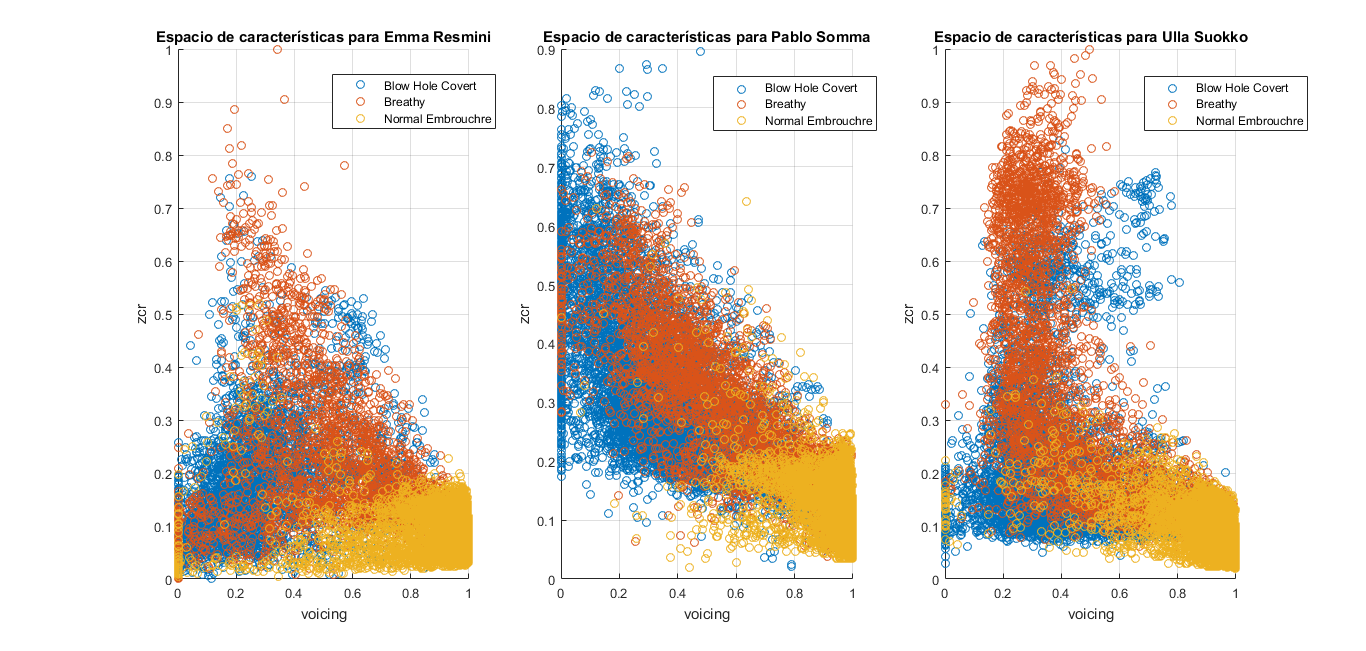
\includegraphics[width=1\textwidth]{histograms_artist} 
%\caption{Espacio de características etiquetado por clases para cada uno de las interpretaciones.}
%\label{fig:histogramas_artista}
%\end{center}
%\end{figure}
%
%\begin{figure}[H]
%\begin{center}
%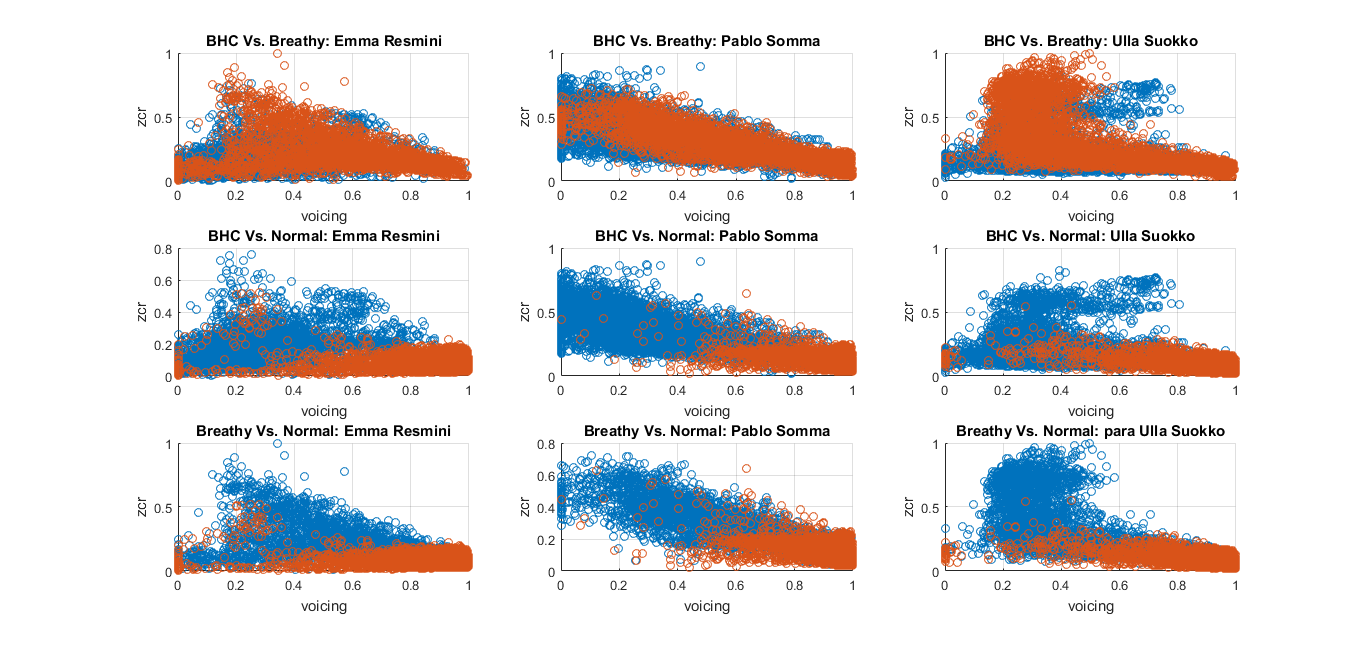
\includegraphics[width=1\textwidth]{comparative} 
%\caption{Comparación clase vs. clase en el espacio de características.}
%\label{fig:comparative}
%\end{center}
%\end{figure}
%
%\newpage
%
%
%Se observa además en las Figuras \ref{fig:bhc_features}, \ref{fig:breathyemb_features} y \ref{fig:normalemb_features} el comportamiento temporal de las características \textit{Voicing} y \textit{Zero-Crossing Rate} superpuestas con el espectrograma, para tres fragmentos de la interpretación de Emma Resmini. Corresponden a \textit{Blow Hole Covered}, \textit{Breathy Embrochure} y \textit{Normal Embrochure} respectivamente. Se corrobora lo dicho anteriormente sobre la separabilidad entre clases.
%
%\begin{figure}[H]
%\begin{center}
%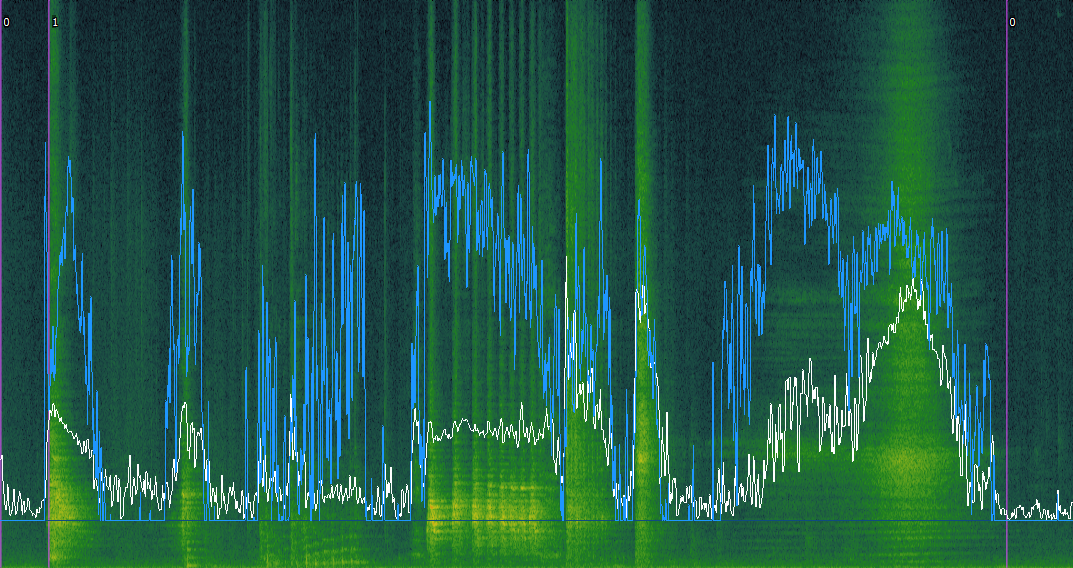
\includegraphics[width=1\textwidth]{bhc_features} 
%\caption{Visualización de un fragmento de la interpretación de Emma Resmini con embocadura \textit{Blow Hole Covered}. Se observa en celeste el \textit{Voicing} y en blanco \textit{Zero-Crossing Rate}.}
%\label{fig:bhc_features}
%\end{center}
%\end{figure}
%
%
%\begin{figure}[H]
%\begin{center}
%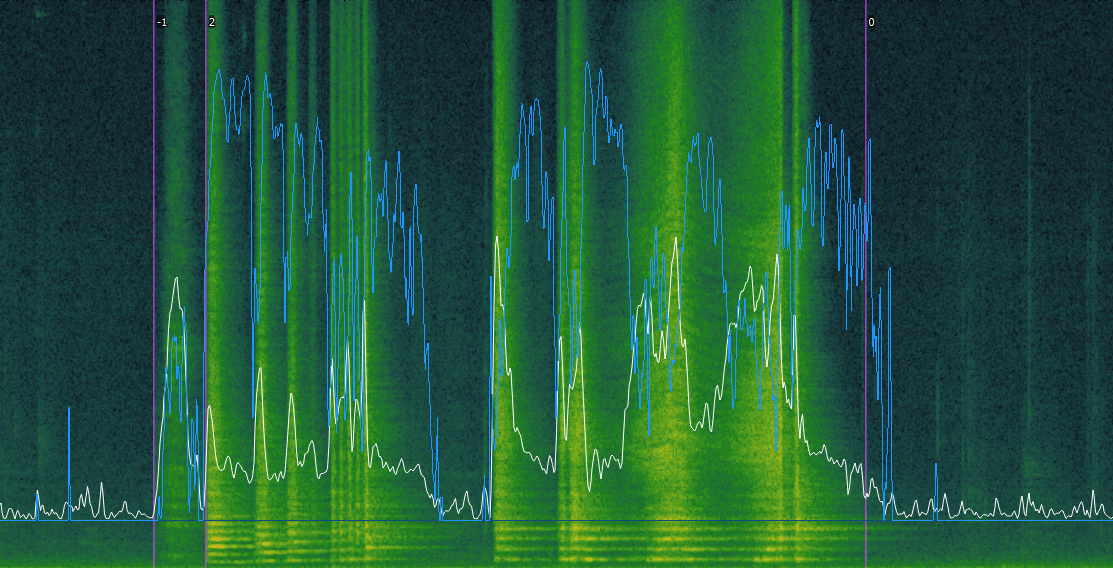
\includegraphics[width=1\textwidth]{breathyemb_features} 
%\caption{Visualización de un fragmento de la interpretación de Emma Resmini con embocadura \textit{Breathy Embrochure}. Se observa en celeste el \textit{Voicing} y en blanco \textit{Zero-Crossing Rate}.}
%\label{fig:breathyemb_features}
%\end{center}
%\end{figure}
%
%
   
\section{Experimentos}
\label{experimento}

Se evalúa la capacidad de los descriptores presentados en la Sección \ref{descriptores} en la separación de embocaduras. Para esto se utilizan tres clasificadores distintos para minimizar el bías que pueda existir entre los datos y un algoritmo en particular. Se trabaja con los algoritmos: \textit{Random Forest (trees=10)}, \textit{Support Vector Machine (kernel lineal)} y \textit{K-Nearest Neighbors (k=10)}. En todos los casos se utilizan los parámetros por defecto ya que no es objetivo de este trabajo encontrar los valores óptimos de clasificación. La implementación se realiza mediante el módulo de \textit{Python} llamado \textit{Scikit Learn} \citep{pedregosa2011scikit}. En todos los casos los datos son preprocesados de manera de centrar en cero y escalar la varianza a uno, previo al clasificador.
\medskip

Todos los experimentos se realizan con \textit{5-fold cross validation} donde los folds son las diferentes interpretaciones de la pieza musical, como se detalla en la Sección \ref{datos}. De esta forma se asegura que frames provenientes de la misma grabación no sean usados para train y test en un mismo experimento. Además los \textit{features}: \textit{MFCC}, \textit{SC}, \textit{Roll-off}, \textit{Centroid}, \textit{ZCR} y \textit{Bandwith} se calculan utilizando el módulo de \textit{Pyhon} llamado \textit{Librosa} \citep{mcfee2015librosa}.
\medskip

\subsection{Primer experimento: Mejor descriptor para extracción de embocadura}
\label{experimento1}

El propósito es cuantificar el poder de separación de las características y determinar cual tiene el mejor desempeño. Para tener una noción general del comportamiento de los descriptores, en todos los casos se utiliza más de una combinación de parámetros. Se eligieron de forma que sea suficiente para descartar los de menor desempeño. A continuación se enlistan los parámetros utilizados en cada caso.

\begin{itemize}
	\item Característcas Espectrales y Armónicas: Se varían los largos de ventana y saltos de la siguiente forma (se detallan respectivamente): (a) $11ms$ y $50\%$ de salto (256-128 muestras), (b) $23ms$ y $50\%$  (1024-512 muestras) y por último (c) $46ms$ y $50\%$  (2048-1024 muestras). En todos los casos anteriores se utilizó: 
	\begin{itemize}
		\item Voicing: Número de retardos: 250 muestras.
		\item Roll-off: $\lambda=85\%$
		\item Centroid, Bandwith y Zero-Crossing Rate: quedan definidos por el largo de la ventana de análisis y el salto.
	\end{itemize}
	\item MFCC: Se computan con ventana de análisis de $23ms$ y salto del $50\%$, 40 bandas Mel y se liftra la señal para obtener: (a) 20 coeficientes, (b) 30 coeficientes y (c) 40 coeficientes.
	\item LPC: Se computan con ventana de análisis de $23ms$ y salto del $50\%$ y numero de polos: (a) 10, (b) 20 y (c) 40.
	\item SC: Se computan con ventana de análisis de $23ms$ y salto del $50\%$ y numero de bandas: (a) 3 y (b) 6.
\end{itemize}

\subsection{Resultados}

En lo que sigue se muestra el resultado del desempeño de los descriptores detallados en la Sección \ref{descriptores} para la extracción del tipo de embocadura.
\medskip

\begin{figure}[H]
\begin{center}
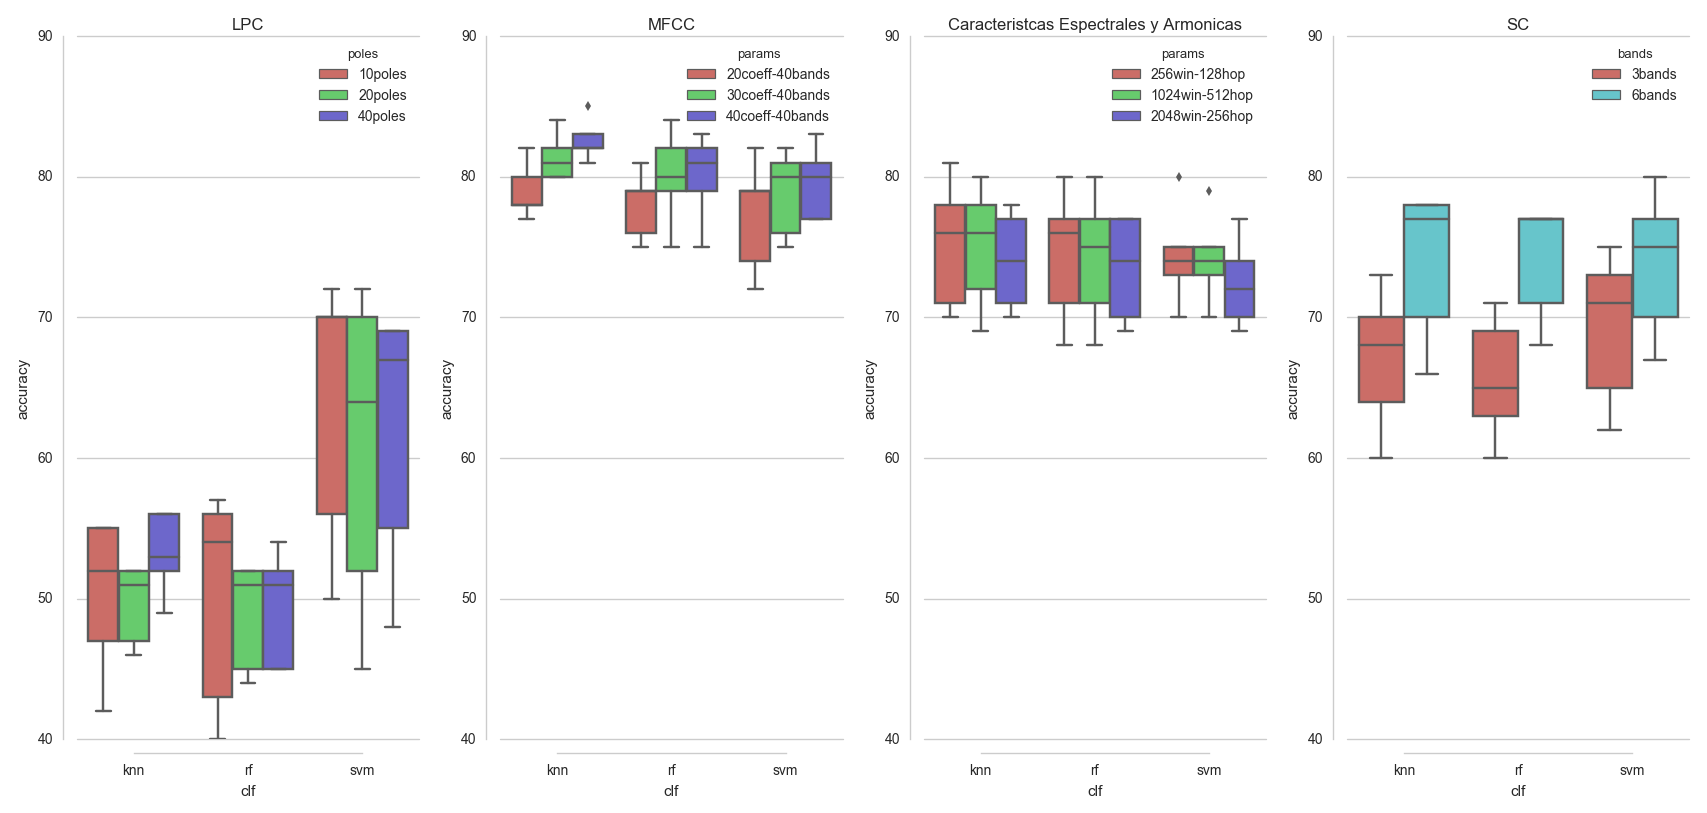
\includegraphics[width=1\textwidth]{exp1_comparacion} 
\caption{Boxplot para el accuracy de los algoritmos de clasificación. Se muestra los resultados de forma independiente por algoritmo de clasificación y según los parámetros de las características.}
\label{fig:exp1_comparacion}
\end{center}
\end{figure}

Se observa en la Figura \ref{fig:exp1_comparacion} el comportamiento de las características en la separación de las clases del problema. Como medida de desmpeño se utiliza la razón entre los frames bien clasificados y el total, deonminada en Inglés como \textit{accuracy}. Además en el eje horizontal se detalla el algoritmo de clasificación utilizado y en colores las distintas combinaciones de parámetros en la extracción de características. 
\medskip

En la Figura \ref{fig:exp1_comparacion} se puede observar claramente que \textit{LPC} es el que presenta peores resultados. Además de forma cualitativa se puede decir que la variación del número de polos del modelo, no afecta considerablemente el desempeño. Como resultado anecdótico a los fines del presente trabajo, se tiene que existe una mejora sustancial en el rendimiento de estos \textit{features} con \textit{SVM}.
\medskip

Por otra parte el \textit{feature} \textit{SC} es de desempeño intermedio junto con \textit{Características Espectrales y Armónicas} en el experimento. Para el caso de \textit{SC} existe una mejora notoria al variar los parámetros. En otras palabras la comparación entre picos y valles tiene un poder descriptivo mayor de el problema, al dividir el espectro en 6 bandas con respecto a 3 bandas.  
\medskip

Del otro lado vemos que la variación de la ventana de análisis en \textit{Características Espectrales y Armónicas} no generan un mejor rendimiento. Vale decir que su desempeño similar al de \textit{SC} pesar de tener dimensiones correlacionadas como es el caso de \textit{ZCR} y \textit{Centroid}. Por lo que alguna estrategia de decorrelación previo al clasificador podría mejorar el desempeño de este conjunto de medidas.
\medskip 

También se observa que \textit{MFCC} es el \textit{feature} de mejor desempeño para la resolución del problema. Como contra partida, frente a \textit{SC} y \textit{Características Espectrales y Armónicas} la dimensión del espacio de características es mayor, resultando en un costo computacional superior. 
\medskip

Otro análisis relevante del experimento esta dado por las matrices de confusión. Para detallar los resultados se deja de lado \textit{LPC} de pobre rendimiento, y se computan las matrices de confusión con la predicción realizada con \textit{KNN} a la grabación de Emma Resmini como conjuto de test. En la Figura \ref{fig:exp1_confusion} se observa las matrices de confusión respectivas, todos los valores son en porcentaje, relativos a la cantidad de frames en la clase.

\begin{figure}[H]
\begin{center}
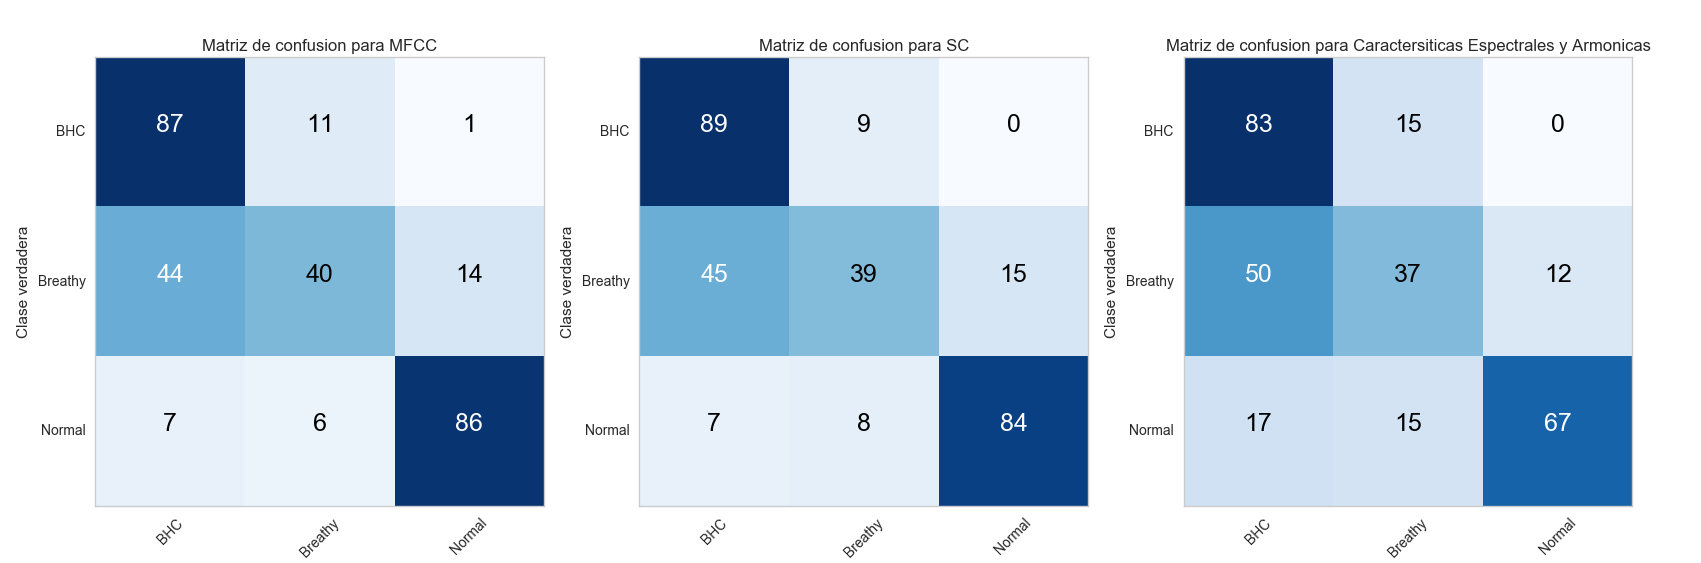
\includegraphics[width=1\textwidth]{exp1_confusion} 
\caption{Matrices de confusión para las características \textit{MFCC}, \textit{SC}, y \textit{Características Espectrales y Armónicas} de izquierda a derecha respectivamente. Para todos los casos el algoritmo de clasificación es KNN.}
\label{fig:exp1_confusion}
\end{center}
\end{figure}

Los resultados demuestran, independientemente de los \textit{features}, que las clases \textit{Blow Hole Covert} y \textit{Normal Embouchure} se separan frente al resto. No es el caso de \textit{Breathy} que principalmente se confunde con \textit{Blow Hole Covert}. Es razonable ya que se puede pensar como el caso intermedio desde el punto de vista acústico, entre las tres clases. Queda planteado entonces el punto débil en la extracción de embocadura de las características propuestas. De ahora en más se trabaja con el \textit{feature} \textit{MFCC} de mejor desempeño. 

%\begin{figure}[H]
%\begin{center}
%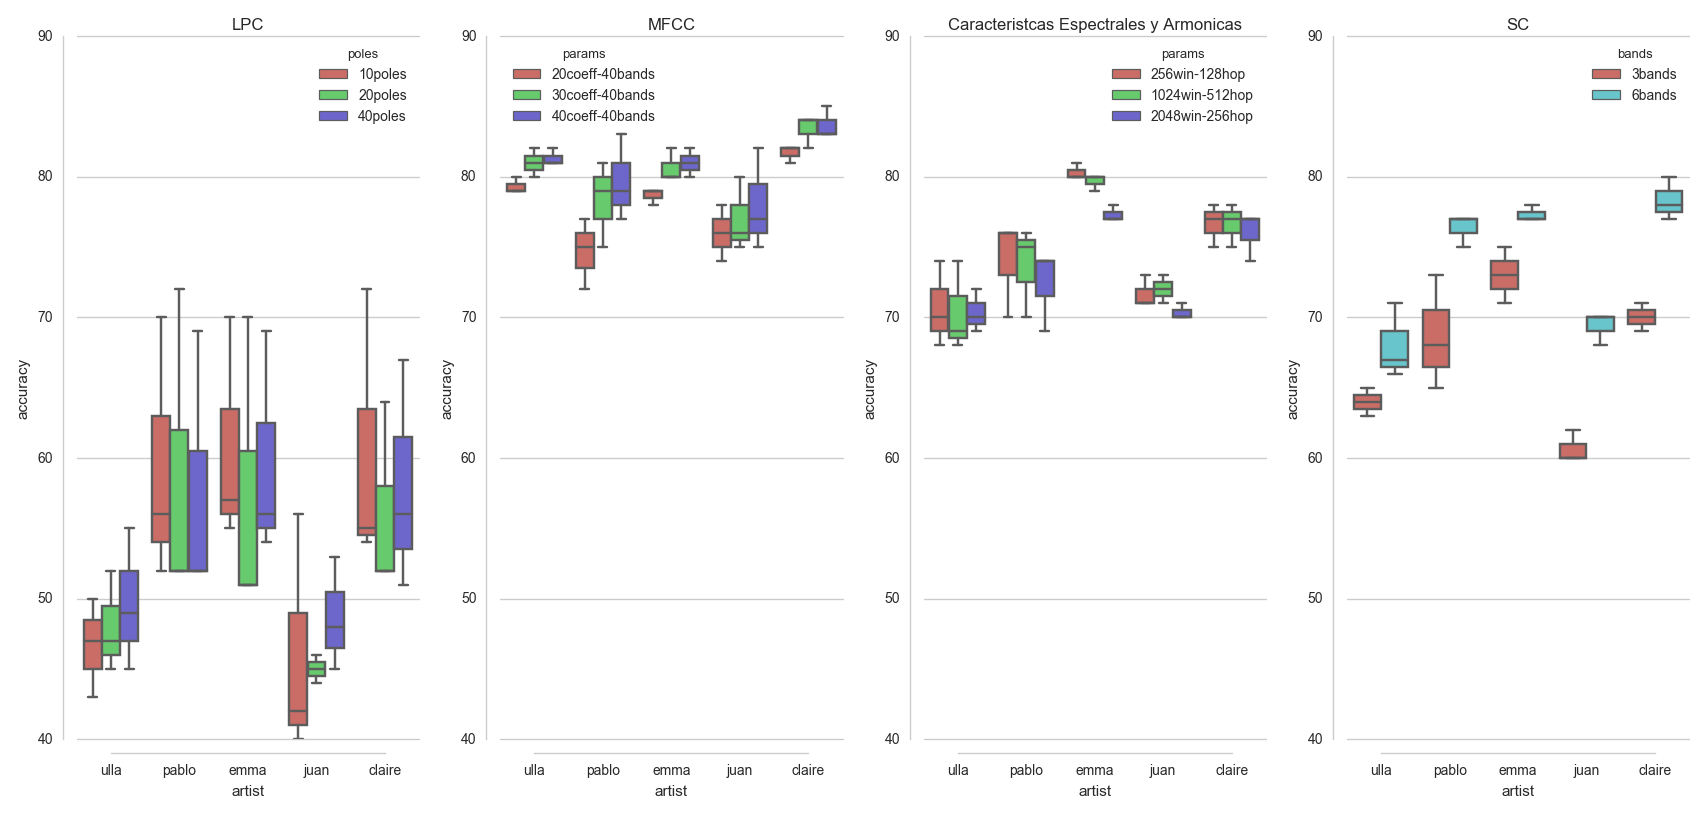
\includegraphics[width=1\textwidth]{exp1_artista} 
%\caption{Boxplot para el accuracy de los algoritmos de clasificación. Se muestra los resultados de forma independiente por artista (fold) y según los parámetros de las características.}
%\label{fig:exp1_artista}
%\end{center}
%\end{figure}

\subsection{Segundo experimento: Blow Hole Covert Vs. Breathy}

En lo que sigue se evalúa nuevamente el desempeño de \textit{MFCC} en la separación de las clases pero con una versión reducida del problema, teniendo en cuenta solamente las dos clases problemáticas: \textit{Blow Hole Covered} y \textit{Breathy Embouchure}. 
\medskip

Por simpleza se trabaja solamente con \textit{MFCC} computado con 40 bandas Mel y 20 coeficientes. En la Figura \ref{fig:exp2_bhcbr} se observa el \textit{accuracy} para los distintos algoritmos de clasificación.

\begin{figure}[H]
\begin{center}
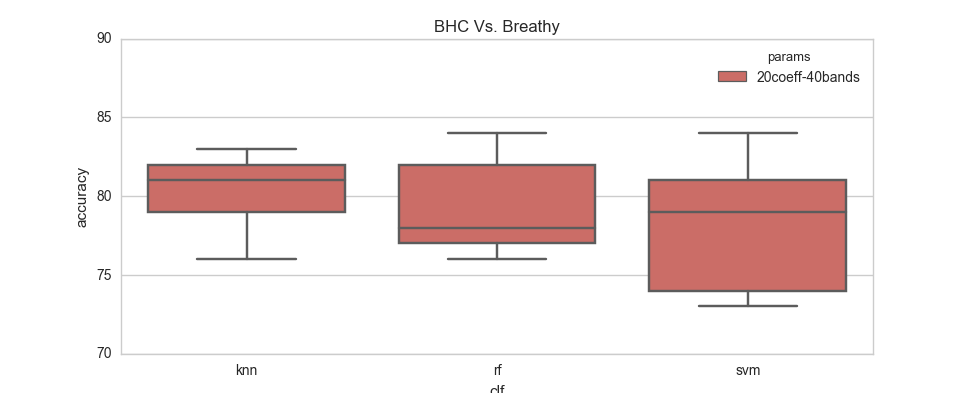
\includegraphics[width=1\textwidth]{exp2_bhcbr} 
\caption{Matrices de confusión para las clases \textit{BHC} Vs. \textit{Breathy} generadas con características MFCC y el clasificador KNN.}
\label{fig:exp2_bhcbr}
\end{center}
\end{figure}

El desempeño es similar al problema completo de tres clases y no existen grandes diferencias en el rendimiento según el algoritmo de clasificación. En la Figura \ref{fig:exp2_confusion} se observa la matriz de confusión para la predicción realizada con \text{KNN} a la grabación de Emma Resmini como conjunto de test, además se normaliza los resultados del experimento de la Sección \ref{experimento1} para realizar la comparación.

\begin{figure}[H]
\begin{center}
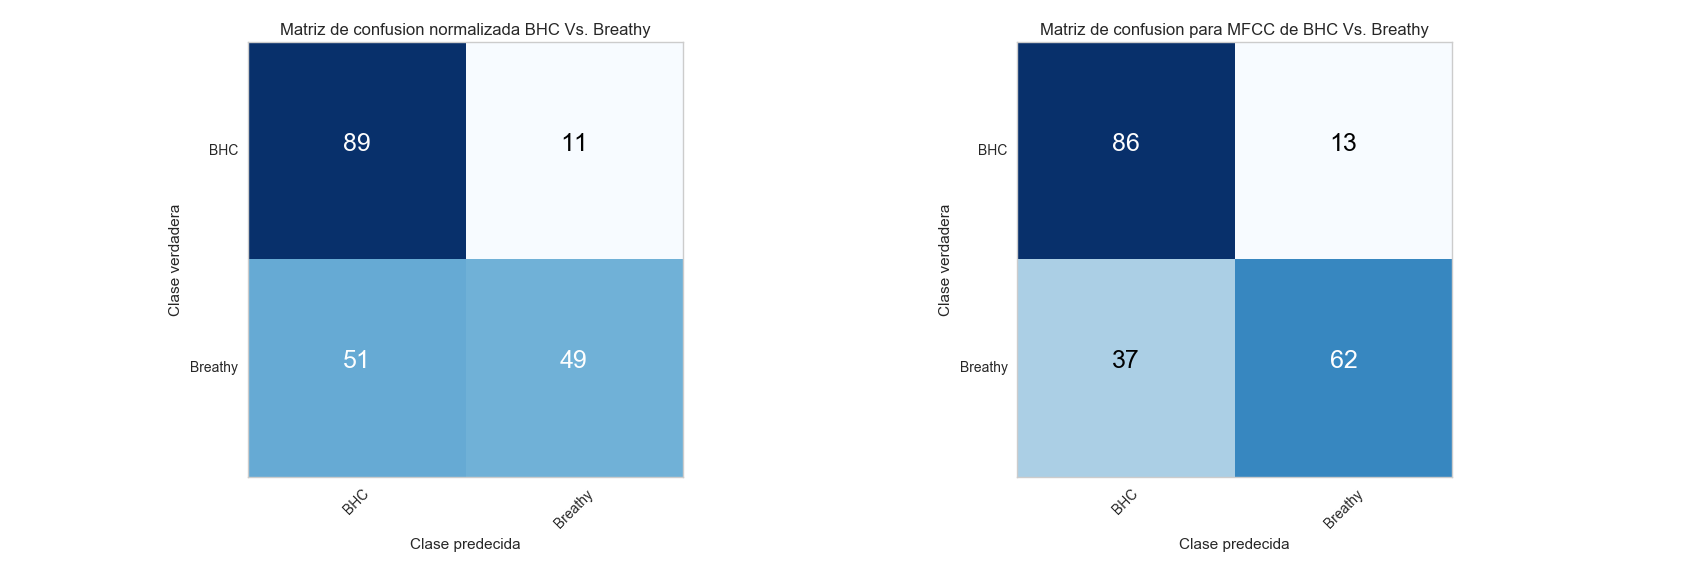
\includegraphics[width=1\textwidth]{exp2_confusion} 
\caption{Matrices de confusión para las clases \textit{BHC} Vs. \textit{Breathy} generadas con características MFCC y el clasificador KNN.}
\label{fig:exp2_confusion}
\end{center}
\end{figure}

Si bien sigue siendo considerable la confusión con un $37\%$ de elementos de \textit{Breathy} clasificados como \textit{Blow Hole Covert}, hay una mejora en comparación al experimento anterior, acertando ahora en la mayoría de los casos. 
\medskip 

Una estrategía de dos estapas de clasificación en cascada mejoraría los resultados con respecto al Experimento \ref{experimento1} a cambio de mayor costo computacional.

\subsection{Refinamiento de la extracción de características basada en MFCC}

En lo que sigue se buscan los parámetros de \textit{MFCC} que logran el resultado óptimo para el problema dado. Recordando la matriz de confusión de la Figura \ref{fig:exp1_confusion}, para el mejor caso (\textit{MFCC} + \textit{KNN}) existe un $13\%$ de frames ejecutados con \textit{Normal Embouchure} que fueron mal clasificados.
\medskip

Mientras \textit{MFCC} es una buena medida del aspecto tímbrico del material sonoro por extraer la envolvente espectral, a priori no contiene información de la periodicidad de la señal de analisis. Por lo que se propone agregar el computo de \textit{Voicing} como una dimensión más del vector de carcterísticas y evaluar si existe disminuición en la confusión de la clase \textit{Normal Embrochure}.
\medskip

\begin{figure}[H]
\begin{center}
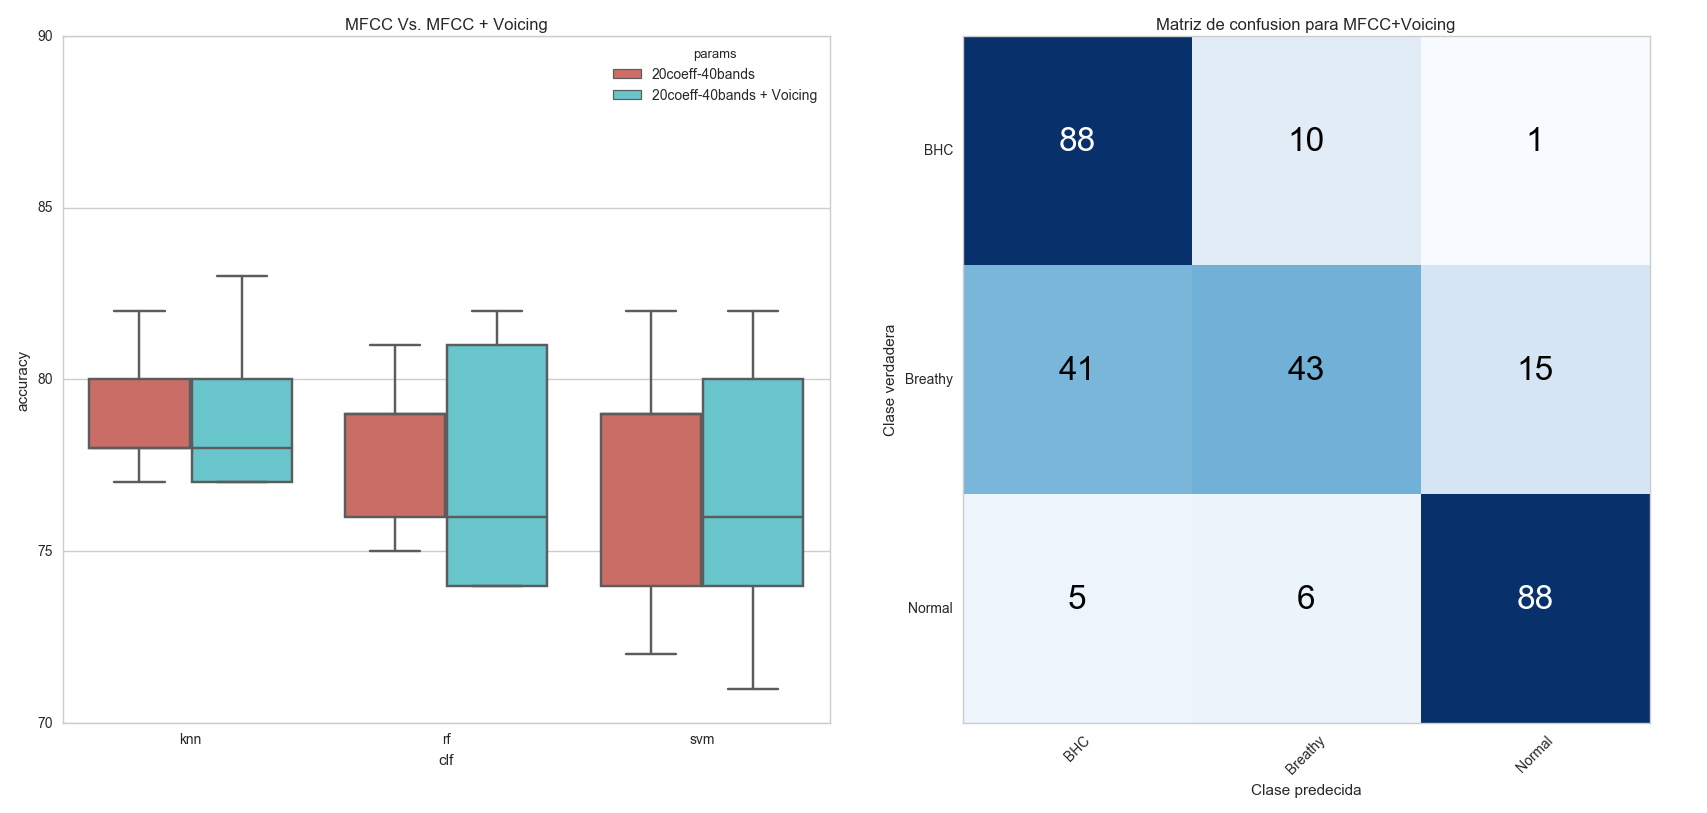
\includegraphics[width=1\textwidth]{exp3} 
\caption{\textit{Accuracy} y matriz de confusión para la evaluación comparativa del agregado de \textit{Voicing} a las características \textit{MFCC}}
\label{fig:exp3}
\end{center}
\end{figure}

Se observa en la Figura \ref{fig:exp3} que tanto el \textit{accuracy}, como la confusión de la clase \textit{Normal Embouchure}, no denotan cambios relevantes de forma cualitativamente.

En lo que sigue se evalúa el desempeño de \textit{MFCC} variando el largo de la vetana de análisis en los valores $11ms$, $23ms$ y $46ms$. En todos los casos el salto entre ventanas es del $50\%$.

\begin{figure}[H]
\begin{center}
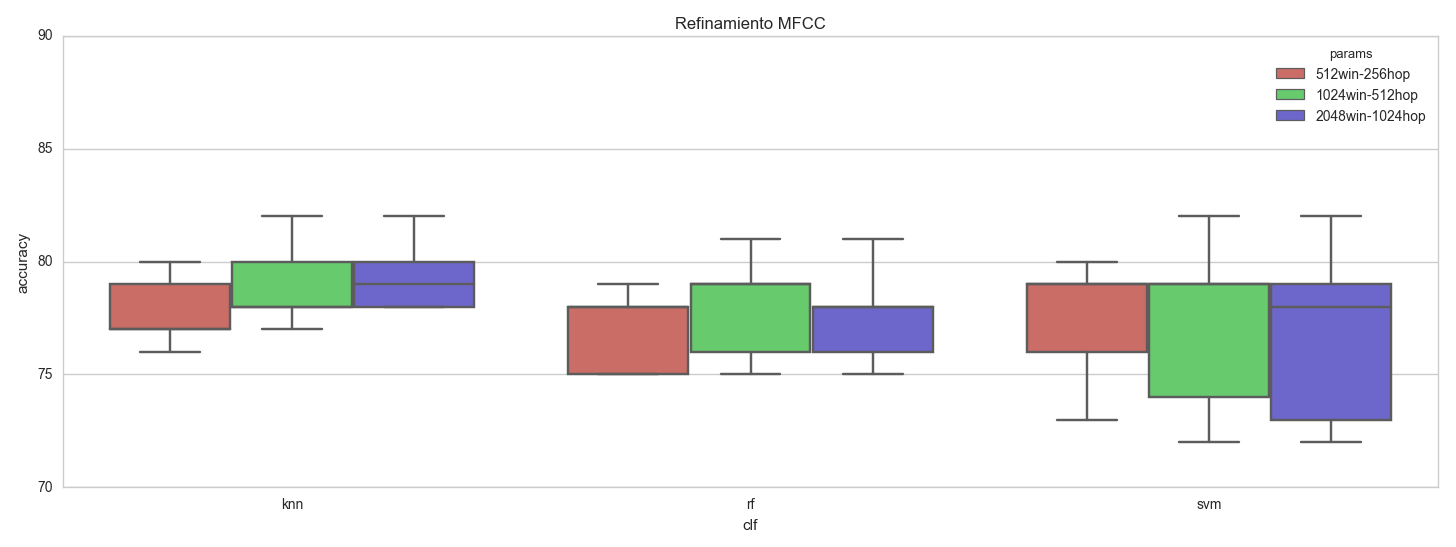
\includegraphics[width=1\textwidth]{exp3_refinamiento} 
\caption{Accuracy de \textit{MFCC} al variar el largo de ventana de análisis.}
\label{fig:exp3_refinmamiento}
\end{center}
\end{figure}

Como se observa en la Figura \ref{fig:exp3_refinmamiento} no existen cambios relevantes en el desempeño al variar el largo de la ventana. Se puede decir que para estos valores la variación tanto en la resolución temporal como en la espectral no es suficiente como para denotar diferencias en el desempeño.  
\medskip

Por ultimo decir que la mejor combinación de parámetros para el cómputo de \textit{MFCC} esta dada por una ventana de $23ms$, 40 bandas Mel y sin liftrado en el dominio de las quefrencys, resultando en un vector 40 dimensiones, siendo alta con respecto a las que se han manejado en el presente trabajo (ver Figura \ref{fig:exp1_comparacion}). Vale restaltar que usualmente se liftra la señal ya que la información tímbrica no se encuentra en las altas quefrencys pero los resultados para estos datos sugieren lo contrario.
\medskip

\newpage

\section{Conclusiones}
\label{conclusiones}
Las características evaluadas en el presente trabajo no fueron adecuadas para la separación de las clases \textit{Blow Hole Covert} y \textit{Breathy}. Con un estudio mas minucioso sobre la naturaleza acústica de estos dos embocaduras se podría diseñar algún \textit{feature} que desambigüe la decisión. 
\medskip

Si bien se concluye que se debe mejorar la separación entre las embocaduras \textit{Blow Hole Covert} y \textit{Breathy}, existen pasajes de transisión, inicios y finales de frases músicales, en los que se vuelve ambigua su naturaleza acústica, y se deben tener en cuenta al momento del etiquetado de las embocaduras. 

\medskip

Desde otro punto de vista la ambiguedad entre las clases sugiere que el enfoque basado en el aspecto tímbrico estimado como la envolvente espectral, no es suficiente. Si bien la embocadura varia el material sonoro y, en un sentido amplio, la composición tímbrica, hay que tener en cuenta que el instrumento físico no cambia. Por lo que el resonador es estacionario y mínima la variación de la estimación de la envolvente espectral a lo largo el tiempo. Esto explicaría por un lado porque los \textit{features} \textit{LPC} tuvieron un pobre desempeño y por otro porque el accuracy óptimo se logra con \textit{MFCC's} sin liftrar. Queda planteada la hipotesis de que la información relevante está en la exitación generada por el intérprete y no por las características del resonador dadas por la envolvente espectral.

\medskip

Por último vale mencionar que la estrategia de \textit{bag of frames} es exigente, ya que se descarta la información temporal de la señal de audio, dejando de lado toda la información a priori. Es mucha la información relevante dada por ser grabaciones de audio de una interpretación musical, de un estilo definido y por si fuera poco con partitura disponible. 


\subsection{Trabajo a futuro}

\begin{itemize} 

  \item Enfocar la resolución del problema desde la estimación de la exitación generada por el intérprete, y evaluar el desempeño con esta estrategia.
  
  \item Segmentación automática del audio en fragmentos de actividad de la flauta y silencios, como primer etapa del sistema de extracción de embocadura, previo a la etapa de clasificación.
   
  \item Salir del bag of frames, para utilizar la redundancia temporal y la información a priori del problema.

\end{itemize}
%----------------------------------------------------------------------------------------
%	BIBLIOGRAPHY
%----------------------------------------------------------------------------------------
\newpage

\section*{Anexo: Representación gráfica de la extracción de embocadura}

A continuación se muestra gráficamente la predicción del clasificador \textit{K-Nearest Neighbors} con las carcterísticas \textit{Mel-Frequency Cepstral Coefficients} con ventana de análisis de $23ms$ y 20 coefficientes computados con 40 bandas Mel. Para la comparación se puede ver también el \textit{ground truth} representado en la mitad izquierda de los rectángulos.
\medskip

La representación se genera asignando a los canales \textit{RGB} de una imagen a color, las probabilidad correspondientes de cada clase a la salida del clasificador. Asignando la probabilidad de \textit{Blow Hole Covert} al canal rojo, \textit{Breathy Embouchure} al verde y el restante \textit{Normal Embouchure} al canal azul se logra el resultado de la Figura \ref{fig:prediccion}.

\bigskip

\begin{figure}[H]
\begin{center}
\includegraphics[width=0.7\textwidth]{prediccion} 
\caption{Representación gráfica de la predicción Vs. el \textit{ground truth}.}
\label{fig:prediccion}
\end{center}
\end{figure}

\newpage
\bibliographystyle{apalike}
\bibliography{biblio}


%----------------------------------------------------------------------------------------
\end{document}


